% !TeX program = xelatex
% !TeX encoding = UTF-8
\documentclass[12pt,a4paper]{article}
\usepackage[margin=2.5cm]{geometry}
\usepackage{amsmath,amssymb}
\usepackage{xeCJK}
\IfFontExistsTF{Microsoft JhengHei}
 {\setCJKmainfont{Microsoft JhengHei}}
 {\setCJKmainfont{FandolSong-Regular}}
\usepackage{booktabs,longtable,array}
\usepackage[hidelinks]{hyperref}
\usepackage{fancyhdr}
\usepackage{enumitem}
\usepackage{graphicx,tikz}
\graphicspath{{images/}{HW2/images/}}
\usetikzlibrary{arrows.meta}
\tikzset{block/.style={draw,minimum height=0.85cm,align=center,font=\footnotesize},sum/.style={draw,circle,inner sep=1pt,minimum size=0.42cm},arr/.style={-{Stealth[length=2mm]},thick}}
\setlist{itemsep=0.3em,topsep=0.4em}
\setlength{\parindent}{0pt}
\setlength{\parskip}{0.3em}
\setlength{\emergencystretch}{2em}
\renewcommand{\arraystretch}{1.18}
\newcolumntype{P}[1]{>{\raggedright\arraybackslash}p{#1}}
\makeatletter
\newcommand{\totalpages}{\@abspage@last}
\makeatother
\pagestyle{fancy}
\fancyhf{}
\renewcommand{\headrulewidth}{0pt}
\fancyfoot[C]{\thepage/\totalpages}
\fancypagestyle{plain}{\fancyhf{}\renewcommand{\headrulewidth}{0pt}\fancyfoot[C]{\thepage/\totalpages}}
\title{Digital Avionics --- Homework 2}
\author{葉彥辰\quad P46154345}
\date{}
\begin{document}
\begin{center}
{\LARGE Digital Avionics --- Homework 2}\\[0.7em]
葉彥辰\quad P46154345\\[0.4em]
CA7528\quad Fall 2026
\end{center}

\section*{Question 1}
Please draw the block diagram of the altitude autopilot for an aircraft and then explain the functions of every part.

\textbf{Solution}

The altitude autopilot adjusts pitch to keep the selected altitude. The inner pitch-rate and pitch-attitude loops respond faster than the outer altitude loop.
\begin{center}
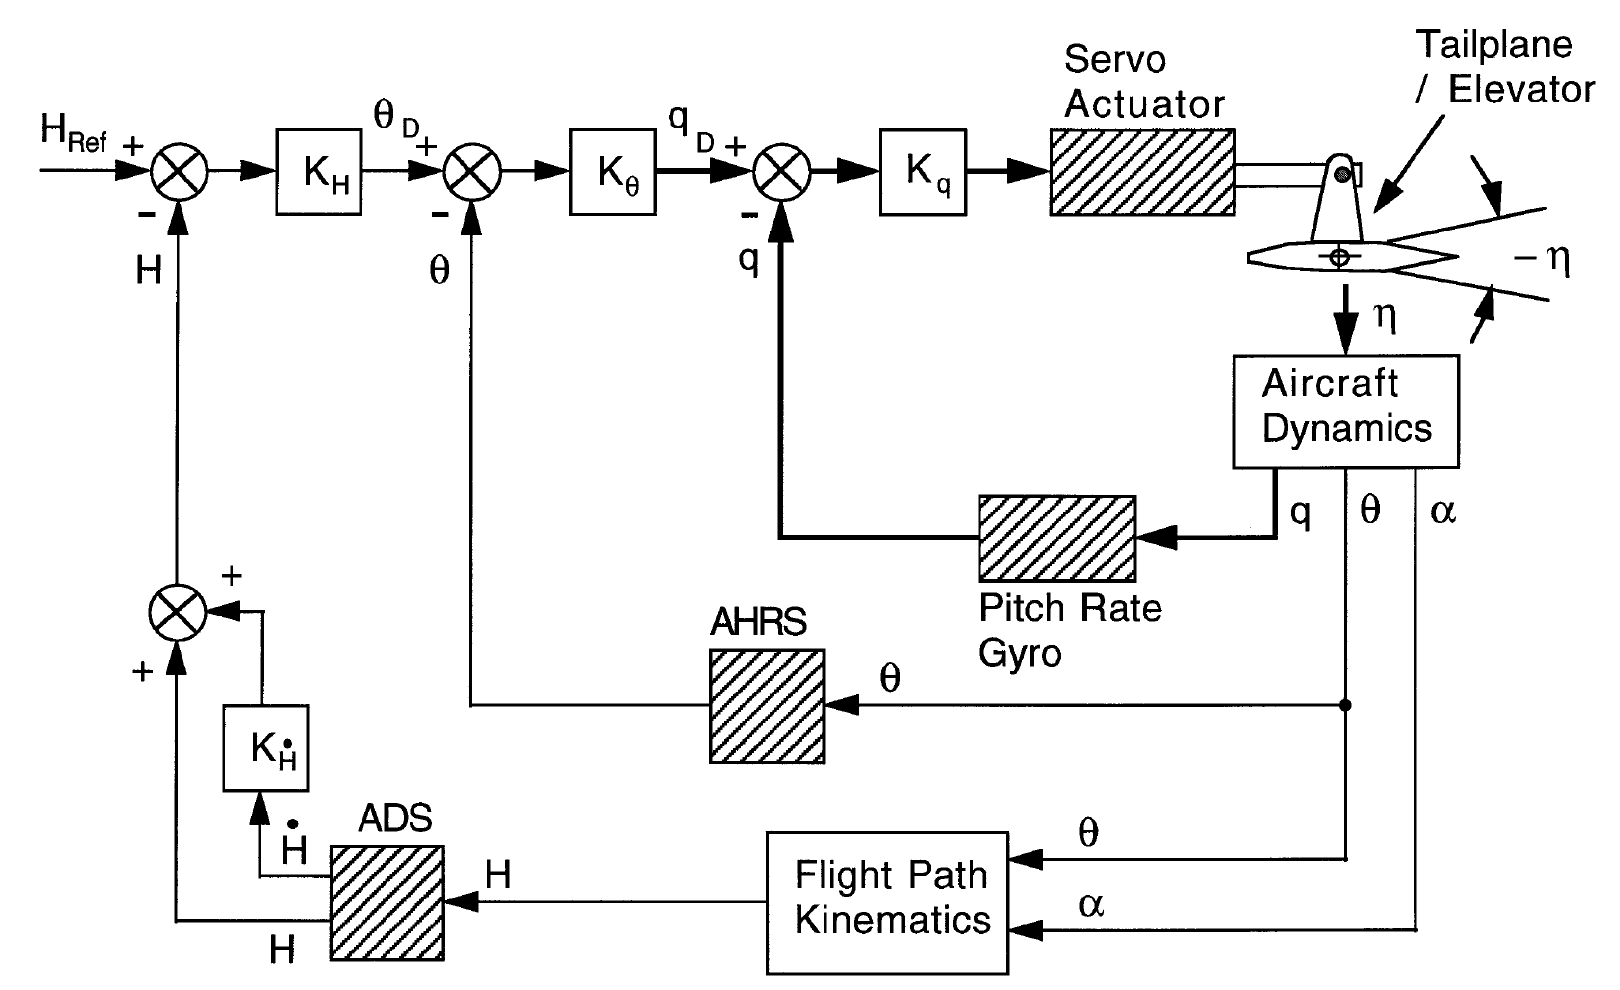
\includegraphics[width=12.0cm]{altitude.png}
\end{center}
\begin{enumerate}[itemsep=0.1em,topsep=0.2em]
\item \textbf{Altitude command and feedback:} $H_{\mathrm{Ref}}$ is the selected altitude. The air data system (ADS) measures altitude $H$ and vertical speed $\dot H$. The $K_{\dot H}\dot H$ feedback helps reduce overshoot during a climb or descent.
\item \textbf{Height gain $K_H$:} The altitude error is converted to a pitch command:
$\theta_D=K_H(H_{\mathrm{Ref}}-H-K_{\dot H}\dot H)$.
\item \textbf{Attitude loop:} The AHRS measures pitch angle $\theta$. The gain $K_\theta$ gives the pitch-rate command $q_D=K_\theta(\theta_D-\theta)$.
\item \textbf{Rate loop:} The pitch-rate gyro measures $q$. The gain $K_q$ acts on $q_D-q$ to make the pitch response fast and well damped.
\item \textbf{Servo and aircraft dynamics:} The servo moves the tailplane/elevator by angle $\eta$. This changes the aircraft's pitch rate, pitch angle, and angle of attack $\alpha$.
\item \textbf{Flight-path kinematics:} Pitch and angle of attack determine the flight-path angle. For small angles and nearly constant speed $V$,
$\dot H\approx V(\theta-\alpha)$. Integrating vertical speed gives altitude, which is fed back through the ADS.
\end{enumerate}
If the aircraft is below the selected altitude, the system commands a climb. As it approaches the target, the feedback reduces the pitch command so that it levels off. Thrust/speed control maintains the required airspeed.
\newpage
\section*{Question 2}
Please draw the block diagram of the heading autopilot for an aircraft and then explain the functions of every part.

\textbf{Solution}

The heading autopilot turns the aircraft toward the selected heading by controlling bank angle. In the diagram, $\Psi$ is heading, $\Phi$ is bank angle, and $p$ is roll rate.
\begin{center}
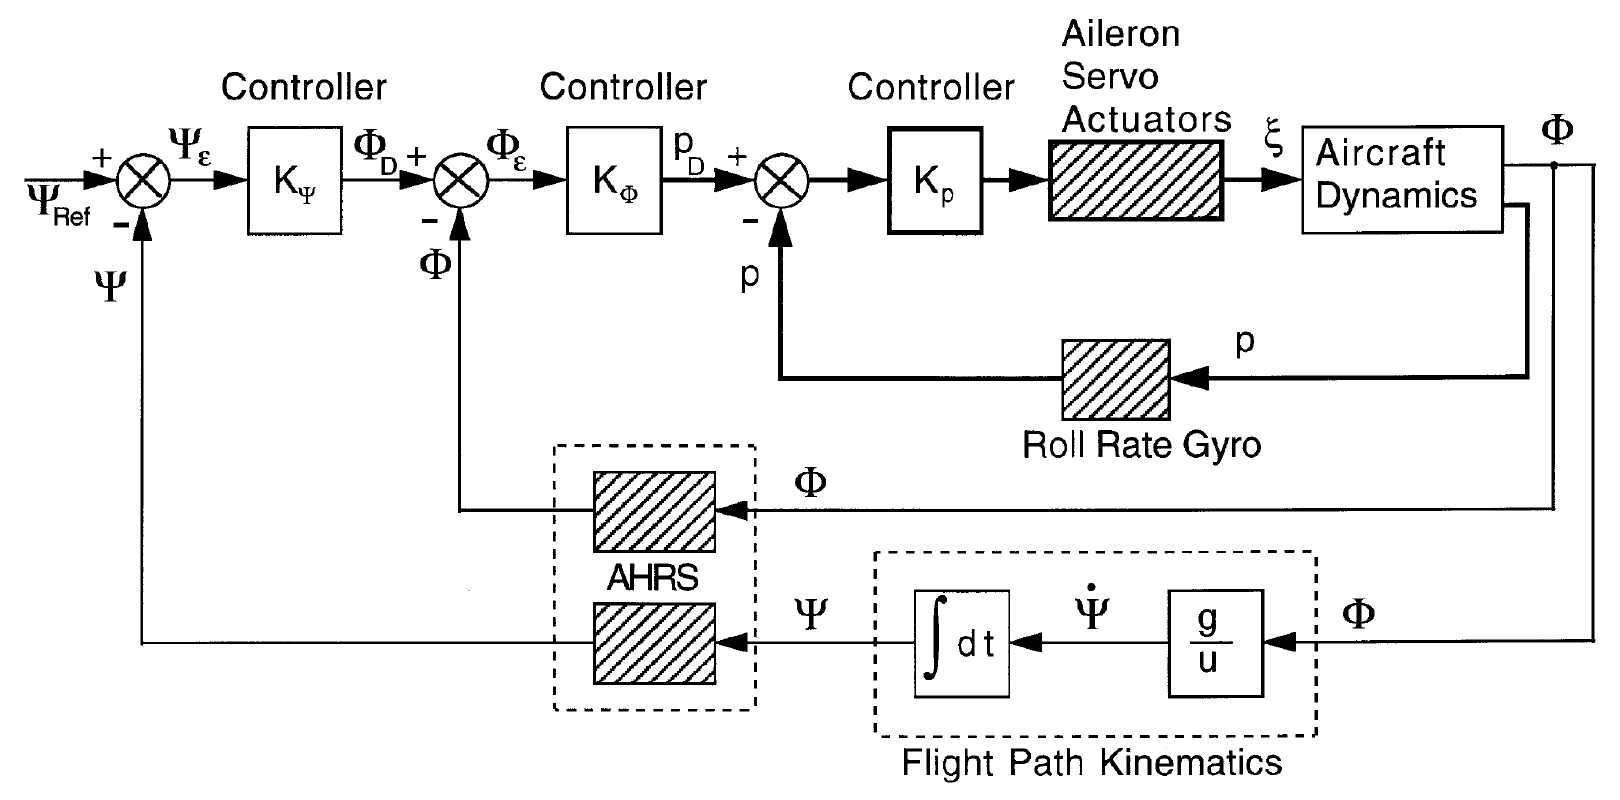
\includegraphics[width=14cm]{heading.png}
\end{center}
\begin{enumerate}
\item \textbf{Heading command and $K_\Psi$:} The selected heading $\Psi_{\mathrm{Ref}}$ is compared with measured heading. The controller gives $\Phi_D=K_\Psi\Psi_e$. The error is taken in the shorter direction; for example, $350^\circ$ to $10^\circ$ is a $20^\circ$ right turn.
\item \textbf{Bank-angle controller $K_\Phi$:} The AHRS measures $\Phi$. The bank error produces a roll-rate command $p_D=K_\Phi(\Phi_D-\Phi)$.
\item \textbf{Roll-rate controller $K_p$:} The roll-rate gyro measures $p$. Feedback of $p_D-p$ gives a fast, well-damped roll response.
\item \textbf{Aileron servo and aircraft dynamics:} The servo moves the ailerons by angle $\xi$. The resulting rolling moment changes roll rate and bank angle.
\item \textbf{Flight-path kinematics:} Banking tilts the lift vector and causes a turn. For a coordinated level turn at forward speed $u$,
\[
\dot\Psi=\frac{g}{u}\tan\Phi\approx\frac{g}{u}\Phi
\quad\text{for small }\Phi.
\]
The $g/u$ block and integrator convert bank angle into heading.
\item \textbf{AHRS feedback:} The AHRS supplies bank angle and heading to the two outer comparison points. These measurements let the autopilot correct the remaining error.
\end{enumerate}
As the heading error decreases, the commanded bank angle returns toward zero and the aircraft rolls level. Rudder coordination helps reduce sideslip, while the altitude loop maintains height. Practical systems also limit bank commands. Holding heading alone does not hold ground track in a crosswind.
\newpage
\section*{Question 3}
Please describe the relationship between stability margin and neutral point.

\textbf{Solution}

The stability margin here is the \textbf{longitudinal static margin}, which tells us how far the CG is ahead of the neutral point. The neutral point (NP) is the centre-of-gravity location at which the pitching-moment coefficient does not change with a small change in angle of attack:
\[
C_{m_\alpha}=\frac{\partial C_m}{\partial\alpha}=0.
\]
Let $x_{CG}$ and $x_{NP}$ be measured aft from the same reference, and let $\bar c$ be the mean aerodynamic chord. The nondimensional positions are $h=x_{CG}/\bar c$ and $h_n=x_{NP}/\bar c$. Then
\[
\boxed{SM=h_n-h=\frac{x_{NP}-x_{CG}}{\bar c}.}
\]
Using positive nose-up pitching moment and $C_{L_\alpha}>0$, the linear relation is
\[
\boxed{C_{m_\alpha}=C_{L_\alpha}(h-h_n)=-C_{L_\alpha}SM.}
\]
\begin{center}
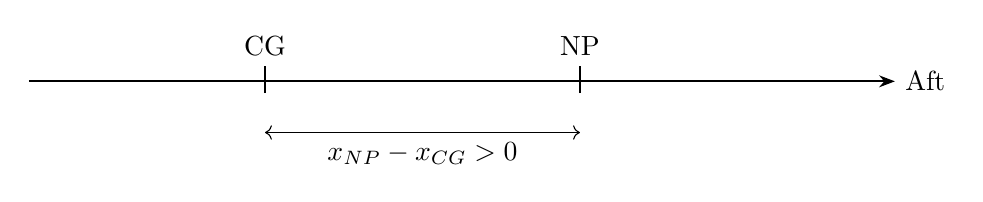
\begin{tikzpicture}[x=1cm,y=1cm]
\draw[arr] (0,0)--(11,0) node[right]{Aft};
\draw (3,-0.15)--(3,0.2) node[above]{CG};
\draw (7,-0.15)--(7,0.2) node[above]{NP};
\draw[<->] (3,-0.65)--node[below]{$x_{NP}-x_{CG}>0$}(7,-0.65);
\end{tikzpicture}
\end{center}
\begin{itemize}
\item \textbf{$SM>0$: CG ahead of NP.} An increase in $\alpha$ produces a restoring nose-down pitching moment. The aircraft is longitudinally statically stable.
\item \textbf{$SM=0$: CG at NP.} There is no first-order restoring moment due to $\alpha$. The aircraft is neutrally stable in this static sense.
\item \textbf{$SM<0$: CG behind NP.} An increase in $\alpha$ produces a nose-up moment that tends to increase the disturbance. Without stability augmentation, the aircraft is statically unstable.
\end{itemize}
For example, if the NP is at $40\%$ MAC and the CG at $30\%$ MAC, then $SM=0.10$, or $10\%$ MAC. Moving the CG aft toward the NP reduces static stability and generally reduces the control effort required to manoeuvre. A larger positive margin increases restoring tendency, but can increase trim and control demands.

The neutral point can change with the aircraft configuration and whether the elevator is fixed or free. The same condition must be used when calculating the static margin. A positive static margin means there is a restoring tendency, but it does not tell us how quickly an oscillation will die out.
\newpage
\section*{Question 4}
Describe the differences between MCAS (Maneuvering Characteristic Augmentation System) and SAS (Stability Augmentation System) of longitudinal motion.

\textbf{Solution}

MCAS and longitudinal SAS both affect the aircraft's pitch motion, but they are used for different purposes.

\textbf{MCAS} is used on the Boeing 737 MAX to reduce the pitch-up tendency at high angle of attack and give the aircraft the intended handling characteristics. It works during manual flight with the flaps up when the angle of attack is high. It commands nose-down stabilizer trim.

\textbf{SAS} improves the aircraft's stability and damping. For example, a pitch-rate gyro detects an unwanted pitching motion, and the SAS moves the elevator or tailplane to oppose it. This helps reduce pitch oscillations after a disturbance.

The main differences are:
\begin{enumerate}
\item \textbf{Purpose:} MCAS mainly changes the handling characteristics at high angle of attack. SAS mainly improves stability and reduces unwanted motion.
\item \textbf{Input:} MCAS uses angle of attack and flight-condition information. A basic longitudinal SAS uses pitch rate $q$. More advanced SAS may also use angle of attack or normal acceleration.
\item \textbf{Output:} MCAS commands nose-down stabilizer trim when its operating conditions are met. SAS commands elevator or tailplane movement in the direction needed to oppose the disturbance.
\item \textbf{Operation:} MCAS works only under specific conditions. SAS provides feedback while it is engaged within its designed operating range, and can also work as an inner loop for an autopilot.
\end{enumerate}
For a simple pitch damper, the stabilizing moment can be represented by
\[
M_{\mathrm{SAS}}=-K_q q,\qquad K_q>0,
\]
where nose-up moment and pitch rate are positive. When the aircraft pitches up, the SAS produces a nose-down moment. When it pitches down, the correction is in the opposite direction.

Therefore, MCAS is a specific handling-augmentation function, while SAS is a more general stability-augmentation system. MCAS is not an altitude-hold autopilot or a complete stall-prevention system.
\newpage
\section*{Question 5}
Explain what is triple redundant system and compare the differences between quadruplex and triple redundant systems.

\textbf{Solution}

A \textbf{triple redundant (triplex) system} has three parallel channels performing the same function. The system compares their outputs and uses majority voting to reject a faulty channel. For example, if A and B give similar outputs but C gives a very different output, C is treated as faulty and disconnected. The other two channels can continue operating.

The diagram below shows the four parallel channels of a quadruplex system.

\begin{center}
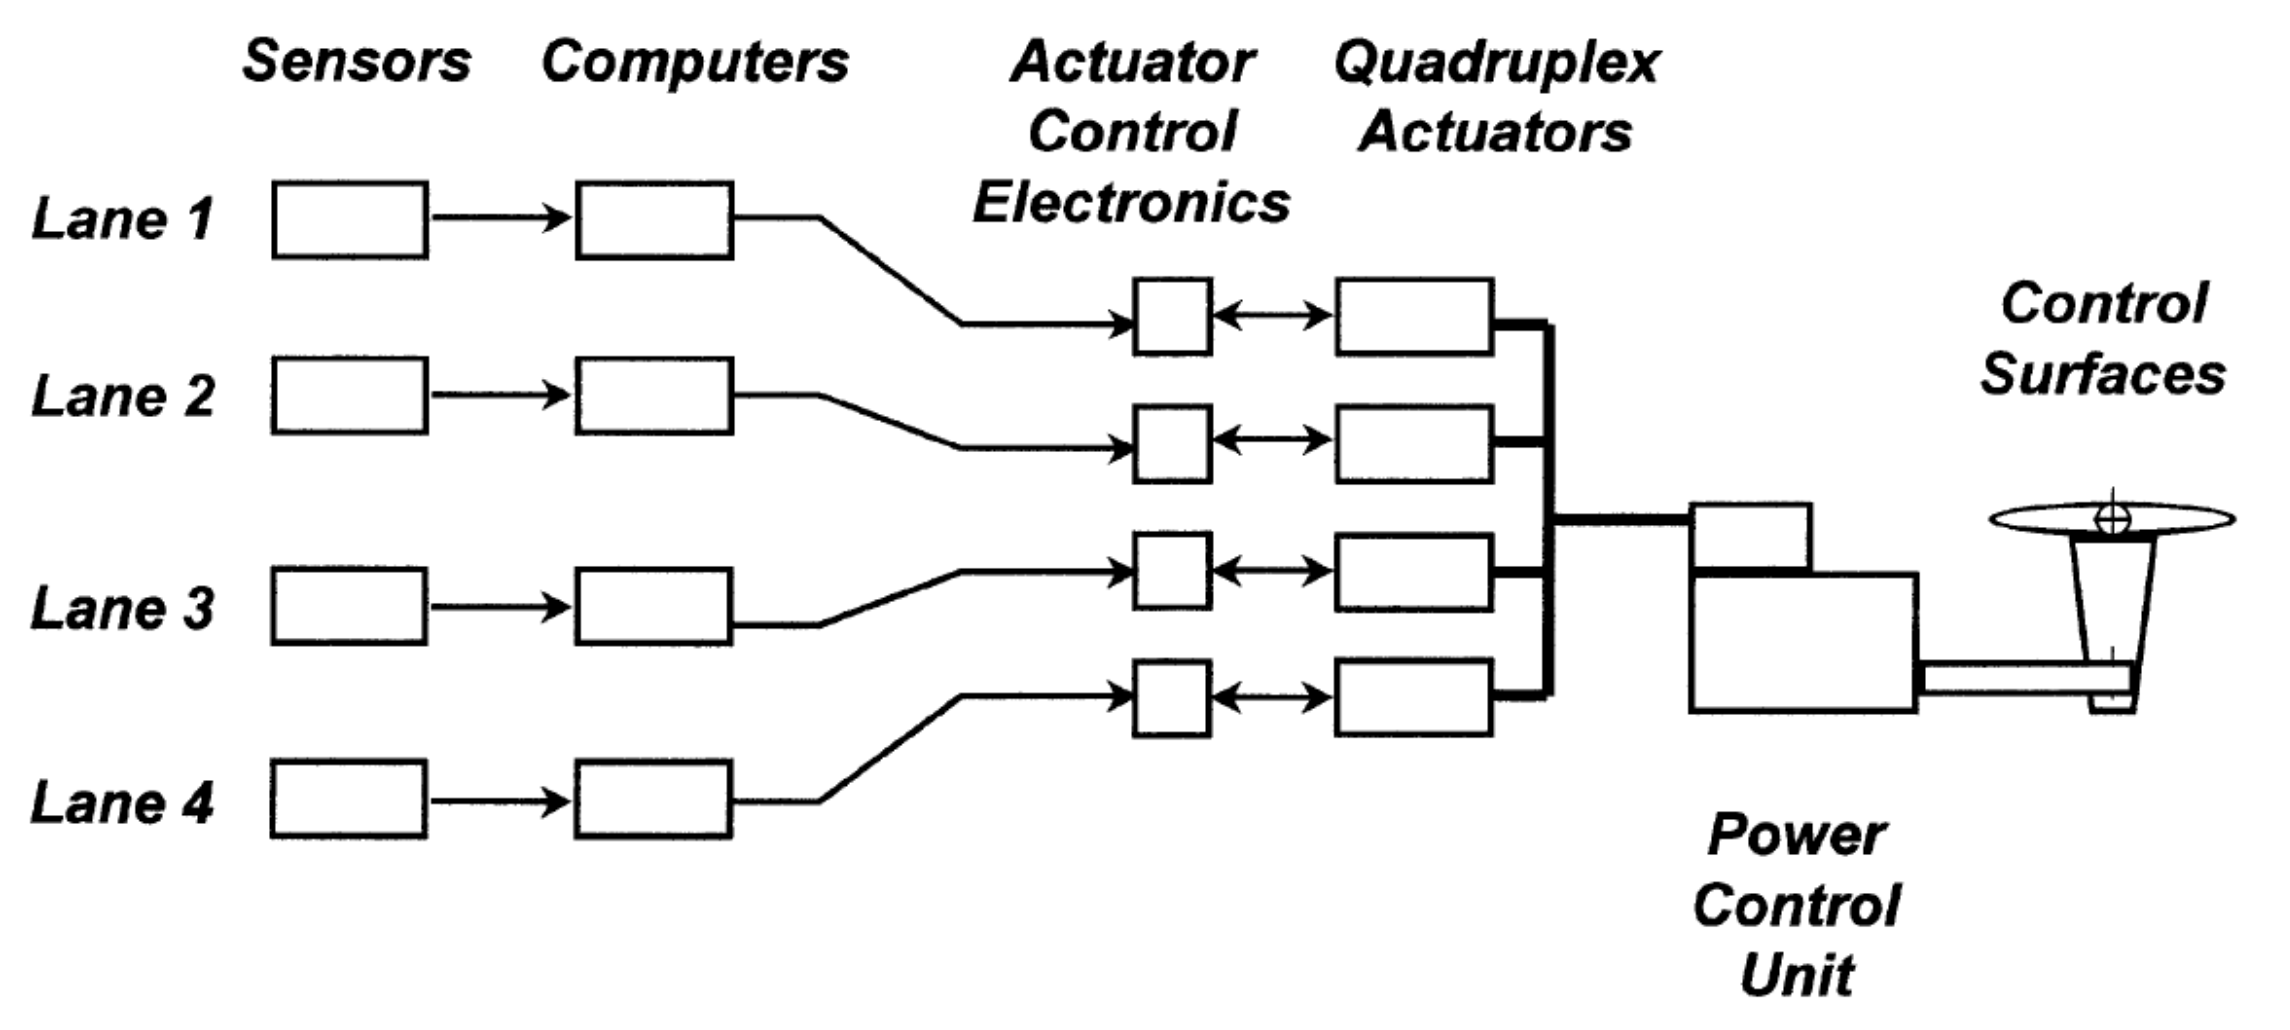
\includegraphics[width=11cm]{redundancy.png}
\end{center}

\small
\begin{tabular}{@{}P{3.0cm}P{5.9cm}P{6.2cm}@{}}
\toprule
Feature & Basic triplex & Quadruplex \\
\midrule
Channel count & Three. & Four. \\
\addlinespace
First independent failure & Two good channels agree, so the faulty one can be disconnected. Two channels remain. & Three good channels agree, so the faulty one can be disconnected. Three channels remain. \\
\addlinespace
Second sequential failure & Two remaining channels can disagree, but comparison alone cannot tell which is correct. & After the first faulty channel is removed, the remaining three can vote again. A second faulty channel can be removed, leaving two. \\
\addlinespace
Typical failure survival & One channel failure by majority voting. & Two separate failures, if each is detected and disconnected in time. \\
\addlinespace
Weight and cost & Less hardware, weight, power use, and cost. & More hardware, weight, and cost, but voting is still available after the first failure. \\
\bottomrule
\end{tabular}
\normalsize

A \textbf{monitored triplex} system is different from basic triplex voting. Each channel has an independent monitor that can identify its own failure. If these monitors are reliable enough, two faulty channels can be disconnected and the system can continue with one good channel.

Quadruplex requires removing the first faulty channel before a second failure creates a two-against-two situation. It cannot handle every pair of simultaneous failures. Both systems need independent power and redundant sensors and actuators, since a shared failure can affect several channels.
\end{document}


